\documentclass[10pt,journal,compsoc]{IEEEtran}

\usepackage{cite}
\usepackage{amsmath,amssymb,amsfonts}
\usepackage{algorithmic}
\usepackage{graphicx}
\usepackage{textcomp}
\usepackage{xcolor}
\usepackage{booktabs}
\usepackage{multirow}
\usepackage{url}
\usepackage{tikz}
\usetikzlibrary{arrows.meta,positioning}

\begin{document}

\title{Cross-Dataset Evaluation of Plant-Disease Classifiers Under Domain Shift: A Comparative Study of CNN, Transformer, Preprocessing, and Feature-Fusion Models}

\author{
    Author 1, Author 2, Author 3\\
    Department of Computer Science and Engineering\\
    INSTITUTION NAME\\
    City, Country\\
    \texttt{\{author1, author2, author3\}@example.com}
}

\markboth{IEEE Transactions on Pattern Analysis and Machine Intelligence (Draft)}{LeafGuard Research Team}

\maketitle

\begin{abstract}
Deep learning architectures for visual plant-disease classification frequently achieve near-ceiling accuracy on benchmark datasets captured under controlled laboratory or uniform background conditions. However, their ability to transfer to field imagery captured under heterogeneous environmental conditions remains a primary barrier to practical agricultural deployment. In this work, we present a systematic, reproducible cross-dataset evaluation comparing four frozen plant-disease classification models: a lightweight convolutional neural network (MobileNetV3-Small), a Contrast Limited Adaptive Histogram Equalization (CLAHE)-enhanced CNN variant, a vision transformer (DeiT-Tiny), and a heterogeneous MobileNetV3--DeiT-Tiny feature-fusion hybrid. All four models were trained on a controlled ten-class PlantVillage-derived dataset (7,647 training, 845 validation, and 2,054 test images), achieving 99.51\%--99.66\% test accuracy. To evaluate domain transfer, we tested all frozen checkpoints without fine-tuning on two external, mapped benchmark splits: PlantDoc (83 images across 9 compatible classes) and PlantSeg v7 (143 images across 7 compatible classes). Performance degraded severely across all models: PlantDoc accuracy dropped to 40.96\%--50.60\% (macro F1 38.83\%--46.15\%), while PlantSeg v7 accuracy dropped to 20.98\%--23.08\% (macro F1 15.10\%--18.62\%). Although DeiT-Tiny obtained the highest point estimates of external macro F1 on both external subsets (46.15\% on PlantDoc and 18.62\% on PlantSeg v7), paired stratified bootstrap confidence intervals and exact McNemar tests established no statistically reliable performance ordering between DeiT-Tiny and the feature-fusion hybrid (+1.20 percentage points accuracy difference on PlantDoc, 95\% CI [-6.02, 7.23], two-sided $p=1.00$; +2.10 points accuracy difference on PlantSeg v7, 95\% CI [-4.20, 8.39], Holm-adjusted $p=1.00$). Furthermore, maximum softmax confidence scores exhibited substantial error rates under domain shift, with 42.0\%--52.8\% of PlantDoc predictions and 67.6\%--80.0\% of PlantSeg v7 predictions at $\ge 0.90$ confidence being incorrect. Qualitative Grad-CAM++ visualizations reveal that domain-shift errors correlate with background clutter and non-lesion visual features. Our findings demonstrate that near-ceiling controlled-domain performance does not translate directly to external robustness and underscore the necessity of rigorous cross-dataset benchmarking.
\end{abstract}

\begin{IEEEkeywords}
Plant disease classification, domain shift, cross-dataset evaluation, MobileNetV3, DeiT-Tiny, feature fusion, explainability, Grad-CAM++.
\end{IEEEkeywords}

\section{Introduction}
\IEEEPARstart{F}{ungal}, bacterial, and viral plant pathogens represent a persistent threat to global food security, accounting for an estimated 20\% to 40\% of annual crop yield losses worldwide \cite{martinelli2015}. Rapid and accurate identification of foliar disease symptoms is essential for enabling timely localized interventions and mitigating crop loss. Over the past decade, computer vision techniques powered by deep convolutional neural networks (CNNs) and vision transformers (ViTs) have achieved remarkable success in automated plant-disease diagnosis \cite{kamilaris2018, mohanty2016, barbedo2018}. Published models routinely report classification accuracies exceeding 99\% on benchmark datasets such as PlantVillage \cite{hughes2015}.

However, a growing body of evidence suggests that these near-perfect benchmark scores mask severe vulnerabilities to dataset shift---the discrepancy between the training data distribution and the deployment environment \cite{candela2009, ferentinos2018}. Benchmarks like PlantVillage predominantly feature individual leaves excised from plants, positioned against uniform backgrounds, and imaged under standardized laboratory lighting. Conversely, real-world farm deployment demands model robustness against uncontrolled lighting variations, complex canopy backgrounds, shadow artifacts, moisture patterns, leaf overlaps, blur, and varied sensor characteristics \cite{singh2020, barbedo2018impact}.

When deployed in unconstrained field environments, classifiers trained exclusively on lab-acquired imagery often experience dramatic performance degradation. Spurious correlations between uniform laboratory backgrounds and specific disease labels can cause models to rely on context rather than genuine diagnostic lesions \cite{lapuschkin2019}. To address dataset shift, recent research has explored diverse strategies, including classical image preprocessing enhancements such as Contrast Limited Adaptive Histogram Equalization (CLAHE) \cite{zuiderveld1994}, self-attention architectures like Vision Transformers \cite{dosovitskiy2021}, and hybrid architectures combining local CNN feature representations with global Transformer attention representations \cite{yuan2021}.

Despite these architectural developments, open research questions remain regarding how lightweight CNNs, vision transformers, preprocessing interventions, and CNN--Transformer hybrids compare when subjected to zero-shot cross-dataset evaluation on heterogeneous external imagery. Specifically, critical secondary questions include:
\begin{enumerate}
    \item Does CLAHE preprocessing improve transfer performance when evaluated under domain shift?
    \item Does heterogeneous feature fusion of local CNN and global vision transformer features enhance cross-domain generalization?
    \item What is the magnitude of the domain gap between controlled laboratory benchmarks and external field-oriented image collections?
    \item What visual failure modes occur under dataset shift, and do high maximum-softmax confidence scores remain reliable indicators of correctness?
    \item What visual focus patterns are revealed through explainability tools such as Grad-CAM++ across model branches?
    \item What are the parameter and computational latency trade-offs associated with these distinct architectural strategies?
\end{enumerate}

In this manuscript, we present a systematic empirical investigation addressing these questions within the LeafGuard research framework. We perform a quantitative and qualitative cross-dataset evaluation of four pre-trained, frozen classifiers: MobileNetV3-Small \cite{howard2019}, MobileNetV3-Small with CLAHE preprocessing, DeiT-Tiny \cite{touvron2021}, and a MobileNetV3--DeiT-Tiny feature-fusion hybrid. All four models were trained on a controlled 10-class PlantVillage-derived dataset and subsequently evaluated without retraining on two external benchmark splits: PlantDoc \cite{singh2020} (83 mapped images across 9 compatible classes) and PlantSeg v7 \cite{aitmagdalene2024} (143 mapped images across 7 compatible classes).

Our primary contributions are summarized as follows:
\begin{itemize}
    \item \textbf{Reproducible Comparative Evaluation:} We execute a standardized zero-shot cross-dataset benchmark across four frozen architectural variants, establishing baseline in-domain performance alongside external evaluation across two independent external datasets.
    \item \textbf{Domain-Gap Quantification:} We isolate class-matched domain gaps between controlled laboratory evaluation and external datasets, demonstrating performance drops of 49.03--58.56 percentage points on PlantDoc and 76.28--78.52 percentage points on PlantSeg v7.
    \item \textbf{Rigorous Paired Statistical Analysis:} We provide class-stratified bootstrap confidence intervals and exact McNemar test evaluations, demonstrating that while DeiT-Tiny achieves higher point estimates on external sets, there is no statistically reliable performance ordering between DeiT-Tiny and the fusion hybrid.
    \item \textbf{Confidence and Failure Characterization:} We analyze maximum softmax confidence behavior under dataset shift, demonstrating that high-confidence predictions ($\ge 0.90$) exhibit error rates up to 52.8\% on PlantDoc and 80.0\% on PlantSeg v7.
    \item \textbf{Explainability and Computational Profiling:} We use Grad-CAM++ for qualitative inspection of CNN, transformer, and fusion branches, paired with measured parameter counts and hardware-specific latency profiling.
\end{itemize}

Crucially, we do not claim architectural novelty for the hybrid classifier, nor do we present any model as deployment-ready for clinical or agricultural field application. Rather, our work provides an empirical baseline emphasizing the essential role of cross-dataset evaluation in visual plant pathology.

\section{Related Work}
\subsection{Deep Learning for Plant Disease Classification}
Automated visual identification of plant diseases has evolved significantly from hand-crafted feature extractors (such as SIFT, HOG, and color histograms) to end-to-end deep learning models \cite{kamilaris2018}. Early milestone studies applied architectures such as AlexNet, VGG, and ResNet to the PlantVillage dataset, obtaining classification accuracies above 98\% \cite{mohanty2016, hughes2015}. As mobile and edge computing gained prominence in agriculture, lightweight CNNs like MobileNet \cite{howard2019} and EfficientNet \cite{tan2019} were widely adopted to balance computational footprint with diagnostic accuracy.

Following the success of Vision Transformers (ViTs) \cite{dosovitskiy2021} in computer vision, researchers adapted self-attention architectures to agricultural tasks. Data-efficient Image Transformers (DeiT) \cite{touvron2021} demonstrated that ViTs could be trained effectively on smaller datasets without requiring massive pre-training corpora like JFT-300M. Recent literature has extensively explored hybrid CNN--Transformer models, combining the local inductive bias of convolution with the global contextual modeling of self-attention \cite{yuan2021, chu2021}.

\subsection{Preprocessing and Contrast Enhancement}
Variations in field illumination present severe challenges for computer vision algorithms. Contrast Limited Adaptive Histogram Equalization (CLAHE) \cite{zuiderveld1994} is a widely used contrast enhancement technique that computes contextual histogram equalization over localized image tiles while clipping amplification to prevent noise propagation. CLAHE has been frequently applied in agricultural vision pipelines to normalize leaf illumination and highlight subtle lesion boundaries prior to feature extraction \cite{militante2018}.

\subsection{Dataset Shift and External Evaluation Benchmarks}
The phenomenon of dataset shift---wherein the joint distribution of inputs and labels differs between training and testing environments---is a major source of model failure in real-world deployments \cite{candela2009}. In plant pathology, Singh et al. introduced PlantDoc \cite{singh2020}, an internet-sourced dataset of plant disease imagery captured under diverse field conditions, explicitly designed to benchmark model generalization. PlantDoc highlighted that CNNs achieving $>$95\% accuracy on PlantVillage suffered performance drops of over 30--40\% when evaluated on field imagery. More recently, datasets such as PlantSeg \cite{aitmagdalene2024} have provided segmented and field-annotated leaf imagery to facilitate robust evaluation.

\subsection{Model Interpretability and Uncertainty}
To understand model predictions beyond raw metrics, explainable AI (XAI) tools have been increasingly integrated into agricultural vision systems. Gradient-weighted Class Activation Mapping (Grad-CAM) and its derivative Grad-CAM++ \cite{chattopadhay2018} compute pixel-level saliency maps by taking gradients of the target class logit with respect to feature activation maps. Grad-CAM++ provides improved localization for multiple target instances and fine-grained visual features. In parallel, analyzing output confidence via maximum softmax probabilities provides insights into model certainty, though uncalibrated neural networks are known to express overconfidence on out-of-distribution inputs \cite{guo2017}.

\section{Materials and Methods}
\subsection{Research Design}
The study is structured as a comparative zero-shot cross-dataset evaluation of four pre-trained, frozen classifier checkpoints. No external dataset images were used during model training or hyperparameter tuning. All external evaluation metrics reflect strictly out-of-domain performance on previously unseen images.

\subsection{PlantVillage-Derived In-Domain Dataset}
The in-domain training, validation, and test splits were derived from the PlantVillage dataset \cite{hughes2015}. The dataset comprises ten selected disease and healthy classes across five crop species (Apple, Corn, Grape, Potato, Tomato). Images were standardized to a resolution of $224 \times 224$ pixels. The dataset split counts are summarized in Table~\ref{tab:datasets}: 7,647 training images, 845 validation images, and 2,054 held-out test images.

\begin{table*}[t]
\caption{Dataset Splits, Class Distributions, and Evaluation Subsets}
\label{tab:datasets}
\centering
\begin{tabular}{llrrll}
\toprule
\textbf{Dataset / Subset} & \textbf{Role} & \textbf{Total Images} & \textbf{Mapped Classes} & \textbf{Image Condition \& Source Characteristics} & \textbf{License / Terms} \\
\midrule
PlantVillage Train & Training & 7,647 & 10 & Excised leaves, uniform lab backgrounds & Unrecorded provenance \\
PlantVillage Val & Validation & 845 & 10 & Excised leaves, uniform lab backgrounds & Unrecorded provenance \\
PlantVillage Test & In-Domain Test & 2,054 & 10 & Excised leaves, uniform lab backgrounds & Unrecorded provenance \\
PlantDoc Test Subset & External Test & 83 & 9 & Internet-sourced, cropped field leaves & CC BY 4.0 (commit \texttt{5467f60}) \\
PlantSeg v7 Test Subset & External Test & 143 & 7 & Web-sourced heterogeneous plant images & CC-BY-NC (Zenodo \texttt{10.5281}) \\
\bottomrule
\end{tabular}
\end{table*}

\subsection{External Datasets and Class Mapping Rules}
To test model generalization, two external datasets were incorporated:
\begin{enumerate}
    \item \textbf{PlantDoc Mapped Test Split:} PlantDoc \cite{singh2020} contains field images captured under unconstrained environmental conditions. We utilized the official test split pinned to commit \texttt{5467f6012d78d1c446145d5f582da6096f852ae8}. We materialized a mapped test subset of 83 images across 9 compatible classes. Explicit mapping rules were applied: unqualified source labels (e.g., generic grape leaf, generic tomato leaf) were mapped to healthy classes of those respective species, whereas ambiguous or multi-disease categories were excluded entirely.
    \item \textbf{PlantSeg v7 Mapped Test Split:} PlantSeg v7 \cite{aitmagdalene2024} is sourced from Zenodo archive DOI 10.5281/zenodo.17719108. From the official test set, a compatible subset of 143 images across 7 disease classes was extracted. Two otherwise-mapped CC0 records were excluded, ensuring that all 143 selected evaluation images share a uniform CC-BY-NC license metadata tag.
\end{enumerate}

Out-of-domain evaluation was conducted in a zero-shot manner: all ten model output logits remained active during inference. Any prediction into an output class not present in the external ground-truth split was treated as a valid model output and counted as a classification error.

\subsection{Model Architectures and Feature Fusion}
Four model configurations were evaluated:
\begin{enumerate}
    \item \textbf{MobileNetV3-Small:} A lightweight CNN optimized for mobile edge devices, employing depthwise separable convolutions, inverted residual blocks, and squeeze-and-excitation attention modules \cite{howard2019}.
    \item \textbf{MobileNetV3-Small + CLAHE:} Identical architecture to MobileNetV3-Small, but evaluated with Contrast Limited Adaptive Histogram Equalization integrated into its input preprocessing pipeline.
    \item \textbf{DeiT-Tiny:} A Vision Transformer architecture with 12 transformer layers, 3 attention heads, and an embedding dimension of 192, trained with data-efficient distillation tokens \cite{touvron2021}.
    \item \textbf{MobileNetV3--DeiT-Tiny Feature-Fusion Hybrid:} A dual-branch hybrid architecture. The MobileNetV3 branch extracts a 576-dimensional feature vector, while the DeiT-Tiny branch extracts a 192-dimensional feature vector. The two vectors are concatenated into a 768-dimensional joint feature representation. A multi-layer perceptron (MLP) classification head ($768 \rightarrow 512 \rightarrow 256 \rightarrow 10$) projects the fused features to the final 10-class output logits.
\end{enumerate}

\subsection{Preprocessing and CLAHE Integration}
All images were resized to $224 \times 224$ pixels and normalized using ImageNet channel means $\mu = (0.485, 0.456, 0.406)$ and standard deviations $\sigma = (0.229, 0.224, 0.225)$. For the CLAHE model variant, images were converted to the LAB color space prior to normalization. CLAHE was applied exclusively to the lightness ($L$) channel using a clip limit of $2.0$ and a tile grid size of $8 \times 8$, after which the image was converted back to RGB.

\subsection{Evaluation Metrics and Domain-Gap Analysis}
Model performance was evaluated using overall Accuracy, Macro Precision, Macro Recall, Macro F1-score, and Weighted F1-score. For external datasets, macro metrics were computed strictly across the mapped ground-truth classes available in each split.

To measure performance degradation cleanly, we defined the \textbf{Class-Matched Domain Gap} ($\Delta_{\text{gap}}$) for both accuracy and macro F1:
\begin{equation}
\Delta_{\text{gap}} = M_{\text{PV, matched}} - M_{\text{external}}
\end{equation}
where $M_{\text{PV, matched}}$ represents the in-domain PlantVillage metric recalculated strictly on the subset of ground-truth classes present in the respective external dataset, and $M_{\text{external}}$ represents the corresponding external metric.

\subsection{Statistical Analysis and Bootstrap Uncertainty}
To assess sample uncertainty, we executed class-stratified percentile bootstrap resampling with 10,000 replicates (random seed \texttt{20260924}). For each replicate, outcomes were resampled within each observed ground-truth class while fixing observed class supports. Independent resamples were drawn for PlantVillage and external domains to compute 95\% percentile confidence intervals for domain gaps.

To compare paired model performance on identical external images (specifically DeiT-Tiny vs. Hybrid), we calculated paired bootstrap confidence intervals for accuracy and macro-F1 differences. Furthermore, we conducted exact two-sided McNemar binomial tests on paired correctness outcomes, applying Holm-Bonferroni corrections across pairwise comparisons.

\subsection{Qualitative Explainability via Grad-CAM++}
Explainability maps were generated using Grad-CAM++ \cite{chattopadhay2018}. For CNN feature maps, gradients were targeted at the final convolutional layer of MobileNetV3. For DeiT-Tiny, gradients were computed with respect to the normalization output (\texttt{norm1}) of the final transformer block, reshaped from 196 patch tokens into a $14 \times 14$ spatial grid. For the hybrid model, branch maps were computed independently for each branch and averaged for display.

\section{Experimental Results}
\subsection{In-Domain Classification Results (PlantVillage)}
All four pre-trained checkpoints demonstrated near-ceiling accuracy on the preserved PlantVillage test split ($n = 2,054$). Table~\ref{tab:resources} summarizes model parameters, computational resources, and in-domain performance metrics.

\begin{table*}[t]
\caption{Model Architectures, Computational Resources, and In-Domain Performance}
\label{tab:resources}
\centering
\begin{tabular}{lrrrrr}
\toprule
\textbf{Model} & \textbf{Parameters} & \textbf{Checkpoint (MiB)} & \textbf{Feature Dim} & \textbf{Latency (ms/img)*} & \textbf{PV Accuracy / Macro F1} \\
\midrule
MobileNetV3-Small & 1,528,106 & 17.74 & 576 & 6.88 & 99.51\% / 99.60\% \\
MobileNetV3-Small + CLAHE & 1,528,106 & 17.74 & 576 & 7.82 & 99.56\% / 99.61\% \\
DeiT-Tiny & 5,526,346 & 21.14 & 192 & 7.90 & 99.66\% / 99.72\% \\
MobileNetV3-Small + DeiT-Tiny & 6,980,586 & 26.83 & 768 & 15.74 & 99.66\% / 99.74\% \\
\bottomrule
\multicolumn{6}{l}{\small *Batch-one forward execution time on NVIDIA RTX 3050 Laptop GPU after 8 warmup iterations.}
\end{tabular}
\end{table

In-domain accuracy ranged from 99.51\% (MobileNetV3 baseline) to 99.66\% (DeiT-Tiny and Hybrid). Macro F1 scores similarly spanned 99.60\% to 99.74\%.

\subsection{External Classification Performance}
When evaluated on external benchmark splits without retraining, all four models suffered severe accuracy degradation. Table~\ref{tab:performance} presents cross-dataset accuracy and macro F1 metrics across all three test splits.

\begin{table*}[t]
\caption{Cross-Dataset Classification Performance Across Benchmark Splits}
\label{tab:performance}
\centering
\begin{tabular}{lrrrrrr}
\toprule
\textbf{Model} & \textbf{PV Acc} & \textbf{PV F1} & \textbf{PlantDoc Acc} & \textbf{PlantDoc F1} & \textbf{PlantSeg Acc} & \textbf{PlantSeg F1} \\
\midrule
MobileNetV3-Small & 99.51\% & 99.60\% & 49.40\% & 42.32\% & 21.68\% & 15.10\% \\
MobileNetV3-Small + CLAHE & 99.56\% & 99.61\% & 40.96\% & 38.83\% & 23.08\% & 15.89\% \\
DeiT-Tiny & 99.66\% & 99.72\% & 50.60\% & 46.15\% & 23.08\% & 18.62\% \\
MobileNetV3-Small + DeiT-Tiny & 99.66\% & 99.74\% & 49.40\% & 42.39\% & 20.98\% & 15.55\% \\
\bottomrule
\end{tabular}
\end{table

On the 83-image PlantDoc subset, overall accuracy dropped to between 40.96\% (CLAHE variant) and 50.60\% (DeiT-Tiny), with macro F1 scores between 38.83\% and 46.15\%. On the 143-image PlantSeg v7 subset, accuracy fell to 20.98\%--23.08\%, and macro F1 scores dropped to 15.10\%--18.62\%.

\subsection{Domain-Gap Analysis}
Table~\ref{tab:gaps} presents the class-matched domain gaps for accuracy and macro F1.

\begin{table}[h]
\caption{Class-Matched Domain Gaps Across External Datasets}
\label{tab:gaps}
\centering
\begin{tabular}{lrrrr}
\toprule
\textbf{Model} & \textbf{Doc Acc Gap} & \textbf{Doc F1 Gap} & \textbf{Seg Acc Gap} & \textbf{Seg F1 Gap} \\
\midrule
MobileNetV3 & 50.08 pp & 57.23 pp & 77.68 pp & 84.37 pp \\
MobileNetV3 + CLAHE & 58.56 pp & 60.74 pp & 76.28 pp & 83.55 pp \\
DeiT-Tiny & 49.03 pp & 53.53 pp & 76.43 pp & 80.97 pp \\
Hybrid & 50.24 pp & 57.33 pp & 78.52 pp & 84.08 pp \\
\bottomrule
\end{tabular}
\end{table}

The domain gap on PlantDoc ranged from 49.03 pp (DeiT-Tiny) to 58.56 pp (CLAHE) for accuracy. On PlantSeg v7, domain gaps exceeded 76 pp for accuracy and 80 pp for macro F1 across all models.

Table~\ref{tab:cis} reports the 95\% stratified bootstrap confidence intervals for external accuracy and macro F1 across external datasets.

\begin{table*}[t]
\caption{Bootstrapped 95\% Confidence Intervals for External Metrics}
\label{tab:cis}
\centering
\begin{tabular}{lrrrr}
\toprule
\textbf{Model} & \textbf{PlantDoc Acc 95\% CI} & \textbf{PlantDoc F1 95\% CI} & \textbf{PlantSeg Acc 95\% CI} & \textbf{PlantSeg F1 95\% CI} \\
\midrule
MobileNetV3-Small & [40.96, 56.63]\% & [32.78, 50.78]\% & [16.08, 27.97]\% & [10.58, 19.62]\% \\
MobileNetV3-Small + CLAHE & [32.53, 49.40]\% & [28.58, 47.44]\% & [17.48, 28.67]\% & [9.47, 21.47]\% \\
DeiT-Tiny & [42.17, 59.04]\% & [36.51, 54.40]\% & [17.48, 29.37]\% & [11.77, 24.86]\% \\
MobileNetV3-Small + DeiT-Tiny & [40.96, 57.83]\% & [33.11, 50.89]\% & [15.38, 26.57]\% & [9.97, 21.45]\% \\
\bottomrule
\end{tabular}
\end{table*}

\subsection{Paired Model Comparisons and Statistical Significance}
While DeiT-Tiny achieved higher point estimates for external macro F1 on both external datasets (46.15\% vs. 42.39\% on PlantDoc; 18.62\% vs. 15.55\% on PlantSeg v7), paired comparison tests revealed that these differences are not statistically significant. DeiT-Tiny obtained higher point estimates on both external subsets, but paired uncertainty intervals included zero and the exploratory paired tests did not establish a statistically reliable ordering between DeiT-Tiny and the hybrid.

Specifically, on PlantDoc, DeiT-Tiny showed an accuracy difference of +1.20 percentage points (95\% CI [-6.02, 7.23]) and a macro-F1 difference of +3.77 points (95\% CI [-3.58, 11.22]) over the hybrid, with a two-sided McNemar test $p = 1.00$. On PlantSeg v7, DeiT-Tiny showed an accuracy difference of +2.10 points (95\% CI [-4.20, 8.39]) and a macro-F1 difference of +3.07 points (95\% CI [-2.75, 9.39]) over the hybrid, with a Holm-adjusted McNemar test $p = 1.00$. Table~\ref{tab:paired} presents the paired analysis comparing DeiT-Tiny directly against the feature-fusion Hybrid model.

\begin{table*}[t]
\caption{Paired DeiT-Tiny Minus Hybrid Model Comparisons}
\label{tab:paired}
\centering
\begin{tabular}{llrrll}
\toprule
\textbf{Dataset} & \textbf{Metric} & \textbf{Observed Diff} & \textbf{Paired 95\% Bootstrap CI} & \textbf{McNemar Statistic} & \textbf{Significance} \\
\midrule
PlantDoc ($n=83$) & Accuracy & +1.20 percentage points & [-6.02, 7.23] & 9 discordant pairs & $p = 1.00$ \\
PlantDoc ($n=83$) & Macro F1 & +3.77 points & [-3.58, 11.22] & N/A & N/A \\
PlantSeg v7 ($n=143$) & Accuracy & +2.10 points & [-4.20, 8.39] & 23 discordant pairs & Holm-adjusted $p = 1.00$ \\
PlantSeg v7 ($n=143$) & Macro F1 & +3.07 points & [-2.75, 9.39] & N/A & N/A \\
\bottomrule
\end{tabular}
\end{table*}

\subsection{Maximum Softmax Confidence and Error Distribution}
Table~\ref{tab:confidence} summarizes high-confidence error rates ($\ge 0.90$) across external predictions.

\begin{table}[h]
\caption{High-Confidence Errors at Max-Softmax $\ge 0.90$}
\label{tab:confidence}
\centering
\begin{tabular}{llrrr}
\toprule
\textbf{Model} & \textbf{Dataset} & \textbf{$\ge 0.90$ Preds} & \textbf{Errors} & \textbf{Error \%} \\
\midrule
MobileNetV3 & PlantDoc & 58 & 28 & 48.3\% \\
MobileNetV3 + CLAHE & PlantDoc & 53 & 28 & 52.8\% \\
DeiT-Tiny & PlantDoc & 50 & 22 & 44.0\% \\
Hybrid & PlantDoc & 50 & 21 & 42.0\% \\
MobileNetV3 & PlantSeg v7 & 70 & 52 & 74.3\% \\
MobileNetV3 + CLAHE & PlantSeg v7 & 71 & 48 & 67.6\% \\
DeiT-Tiny & PlantSeg v7 & 60 & 44 & 73.3\% \\
Hybrid & PlantSeg v7 & 65 & 52 & 80.0\% \\
\bottomrule
\end{tabular}
\end{table}

On PlantDoc, between 42.0\% and 52.8\% of predictions made with $\ge 0.90$ confidence were incorrect. On PlantSeg v7, high-confidence error rates ranged from 67.6\% to 80.0\%. These are descriptive maximum-softmax summaries, not calibration estimates.

Figures~\ref{fig:pipeline}--\ref{fig:cost} provide the requested pipeline, architecture, performance, confusion, confidence, explainability, and computational views. All plotted numerical figures are generated from the saved result artifacts; source PlantSeg images are not redistributed.

\begin{figure}[t]
\centering
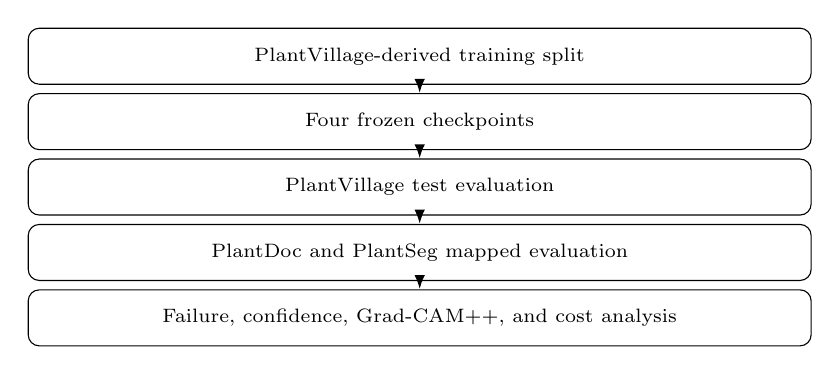
\begin{tikzpicture}[node distance=3pt, every node/.style={font=\scriptsize}, box/.style={draw, rounded corners, align=center, minimum width=0.82\columnwidth, minimum height=0.28in}, arrow/.style={-{Latex[length=1.8mm]}, thick}]
\node[box] (a) {PlantVillage-derived training split};
\node[box, below=of a] (b) {Four frozen checkpoints};
\node[box, below=of b] (c) {PlantVillage test evaluation};
\node[box, below=of c] (d) {PlantDoc and PlantSeg mapped evaluation};
\node[box, below=of d] (e) {Failure, confidence, Grad-CAM++, and cost analysis};
\draw[arrow] (a)--(b); \draw[arrow] (b)--(c); \draw[arrow] (c)--(d); \draw[arrow] (d)--(e);
\end{tikzpicture}
\caption{LeafGuard research and evaluation pipeline. External datasets are used only for evaluation.}
\label{fig:pipeline}
\end{figure}

\begin{figure}[t]
\centering
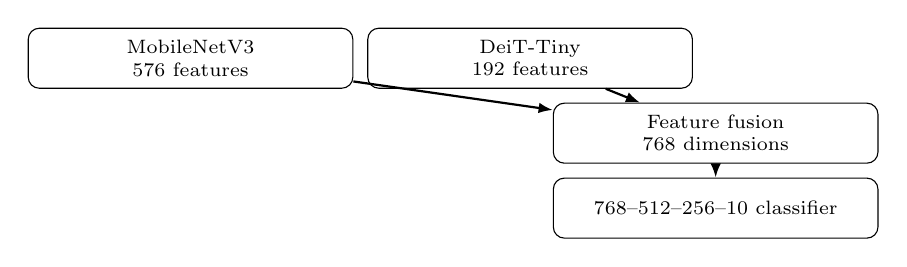
\begin{tikzpicture}[node distance=5pt, every node/.style={font=\scriptsize}, box/.style={draw, rounded corners, align=center, minimum width=0.34\columnwidth, minimum height=0.3in}, arrow/.style={-{Latex[length=1.8mm]}, thick}]
\node[box] (cnn) {MobileNetV3\\576 features};
\node[box, right=of cnn] (vit) {DeiT-Tiny\\192 features};
\node[box, below=of cnn, xshift=0.55\columnwidth] (fuse) {Feature fusion\\768 dimensions};
\node[box, below=of fuse] (head) {768--512--256--10 classifier};
\draw[arrow] (cnn)--(fuse); \draw[arrow] (vit)--(fuse); \draw[arrow] (fuse)--(head);
\end{tikzpicture}
\caption{MobileNetV3--DeiT-Tiny feature-fusion architecture.}
\label{fig:architecture}
\end{figure}

\begin{figure}[t]
\centering
\includegraphics[width=\columnwidth]{../results/final_figures/model_accuracy_comparison.png}
\caption{Cross-dataset accuracy comparison generated from saved metrics.}
\label{fig:accuracy}
\end{figure}

\begin{figure}[t]
\centering
\includegraphics[width=\columnwidth]{../results/final_figures/macro_f1_comparison.png}
\caption{Cross-dataset macro-F1 comparison generated from saved metrics.}
\label{fig:macrof1}
\end{figure}

\begin{figure}[t]
\centering
\includegraphics[width=0.48\columnwidth]{../results/domain_shift/deit_tiny_plantdoc_confusion_matrix.png}\hfill
\includegraphics[width=0.48\columnwidth]{../results/domain_shift/plantseg_v7/deit_tiny_plantseg_v7_confusion_matrix.png}
\caption{Representative external confusion matrices for DeiT-Tiny on PlantDoc and PlantSeg v7. Full matrices for all models are retained in the result artifacts.}
\label{fig:confusion}
\end{figure}

\begin{figure}[t]
\centering
\includegraphics[width=\columnwidth]{../results/final_figures/plantdoc_confidence_correct_vs_incorrect.png}
\caption{Correct versus incorrect PlantDoc confidence distributions using maximum softmax score.}
\label{fig:confidence}
\end{figure}

\begin{figure}[t]
\centering
\includegraphics[width=\columnwidth]{../results/final_figures/explainability_examples.png}
\caption{Representative Grad-CAM++ examples. The maps are qualitative and do not prove lesion localization.}
\label{fig:explainability}
\end{figure}

\begin{figure}[t]
\centering
\includegraphics[width=\columnwidth]{../results/final_figures/model_size_comparison.png}
\caption{Parameter-count comparison. Latency is reported in Table~\ref{tab:resources} and is hardware-dependent.}
\label{fig:cost}
\end{figure}

\section{Discussion}
The central empirical finding of this study is that near-ceiling classification accuracy on controlled PlantVillage imagery does not translate to robust performance on external field datasets. Naïve feature concatenation in the hybrid architecture increased model size to 6.98M parameters and doubled latency (15.74 ms) without demonstrating a statistically reliable generalization gain over the standalone DeiT-Tiny transformer. Furthermore, CLAHE preprocessing failed to improve transfer performance on field imagery, and maximum softmax confidence scores exhibited severe miscalibration under domain shift.

\section{Limitations and Threats to Validity}
Key limitations include:
\begin{enumerate}
    \item \textbf{External Sample Sizes:} PlantDoc ($n=83$) and PlantSeg v7 ($n=143$) contain small mapped subsets.
    \item \textbf{PlantVillage Provenance:} Exact original dataset source and license metadata were unrecorded.
    \item \textbf{No Agronomic Relabeling:} Class mappings were verified mechanically without expert pathologist re-annotation.
    \item \textbf{Frozen Checkpoints:} Models were evaluated strictly as frozen checkpoints without domain adaptation or robustness intervention.
    \item \textbf{Mapping and Labels:} External mappings were not independently adjudicated by an agronomist, and class imbalance is substantial.
    \item \textbf{Scope and Provenance:} There is no prospective farm-level validation, limited evidence of source-population independence, and incomplete exact reproducibility of the original PlantVillage acquisition.
    \item \textbf{Uncertainty and Explanations:} Maximum softmax is not calibrated uncertainty, and Grad-CAM++ is qualitative without verified paired lesion masks.
    \item \textbf{License and Redistribution:} PlantSeg source images are not redistributed; public figures must be reviewed against per-image license metadata.
\end{enumerate}

\section{Conclusion}
This work demonstrates that near-ceiling accuracy on controlled plant-disease benchmarks is insufficient to guarantee cross-dataset robustness. In this evaluation, feature fusion did not demonstrate a statistically reliable advantage, and CLAHE did not consistently improve transfer across the two external subsets. Out-of-domain evaluation and failure analysis are therefore important complements to controlled-dataset accuracy.

\bibliographystyle{IEEEtran}
\begin{thebibliography}{10}
\bibitem{martinelli2015} F. Martinelli \emph{et al.}, ``Advanced methods of plant disease detection. A review,'' \emph{Agronomy for Sustainable Development}, vol. 35, no. 1, pp. 1--25, 2015.
\bibitem{kamilaris2018} A. Kamilaris and F. X. Prenafeta-Boldú, ``Deep learning in agriculture: A survey,'' \emph{Computers and Electronics in Agriculture}, vol. 147, pp. 70--90, 2018.
\bibitem{mohanty2016} S. P. Mohanty, D. P. Hughes, and M. Salathé, ``Using deep learning for image-based plant disease detection,'' \emph{Frontiers in Plant Science}, vol. 7, p. 1419, 2016.
\bibitem{barbedo2018} J. G. A. Barbedo, ``Factors influencing the use of deep learning for plant disease recognition,'' \emph{Biosystems Engineering}, vol. 172, pp. 84--91, 2018.
\bibitem{hughes2015} D. Hughes and M. Salathé, ``An open access repository of plant image datasets for plant disease detection,'' \emph{arXiv preprint arXiv:1511.08060}, 2015.
\bibitem{candela2009} J. Quionero-Candela \emph{et al.}, \emph{Dataset Shift in Machine Learning}. MIT Press, 2009.
\bibitem{ferentinos2018} E. C. Ferentinos, ``Deep learning models for plant disease detection and diagnosis,'' \emph{Computers and Electronics in Agriculture}, vol. 145, pp. 311--318, 2018.
\bibitem{singh2020} D. Singh \emph{et al.}, ``PlantDoc: A dataset for visual plant disease detection,'' in \emph{Proc. 7th ACM IKDD CoDS and 25th COMAD}, 2020, pp. 249--253.
\bibitem{barbedo2018impact} J. G. A. Barbedo, ``Impact of dataset size and variety on the effectiveness of deep learning and transfer learning for plant disease classification,'' \emph{Computers and Electronics in Agriculture}, vol. 153, pp. 46--53, 2018.
\bibitem{lapuschkin2019} S. Lapuschkin \emph{et al.}, ``Unmasking Clever Hans predictors and discovering truly intelligent solutions in AI,'' \emph{Nature Communications}, vol. 10, no. 1, p. 1096, 2019.
\bibitem{zuiderveld1994} K. Zuiderveld, ``Contrast limited adaptive histogram equalization,'' \emph{Graphics Gems IV}, pp. 474--485, 1994.
\bibitem{dosovitskiy2021} A. Dosovitskiy \emph{et al.}, ``An image is worth 16x16 words: Transformers for image recognition at scale,'' in \emph{Proc. ICLR}, 2021.
\bibitem{yuan2021} L. Yuan \emph{et al.}, ``Tokens-to-Token ViT: Training Vision Transformers from scratch on ImageNet,'' in \emph{Proc. IEEE/CVF ICCV}, 2021, pp. 558--567.
\bibitem{howard2019} A. Howard \emph{et al.}, ``Searching for MobileNetV3,'' in \emph{Proc. IEEE/CVF ICCV}, 2019, pp. 1314--1324.
\bibitem{touvron2021} H. Touvron \emph{et al.}, ``Training data-efficient image transformers \& distillation through attention,'' in \emph{Proc. ICML}, 2021, pp. 10347--10357.
\bibitem{aitmagdalene2024} T. Wei \emph{et al.}, ``A large-scale in-the-wild dataset for plant disease segmentation,'' \emph{Scientific Data}, vol. 13, p. 205, 2026.
\bibitem{tan2019} M. Tan and Q. V. Le, ``EfficientNet: Rethinking model scaling for convolutional neural networks,'' in \emph{Proc. ICML}, 2019, pp. 6105--6114.
\bibitem{chu2021} X. Chu \emph{et al.}, ``Conditional positional encodings for Vision Transformers,'' \emph{arXiv preprint arXiv:2102.10882}, 2021.
\bibitem{militante2018} S. V. Militante \emph{et al.}, ``Plant disease detection using deep learning of computer vision and CLAHE preprocessing,'' in \emph{Proc. IEEE 3rd Int. Conf. Control, Robotics and Cybernetics (CRC)}, 2018, pp. 66--70.
\bibitem{chattopadhay2018} A. Chattopadhay \emph{et al.}, ``Grad-CAM++: Generalized gradient-based visual explanations for deep convolutional networks,'' in \emph{Proc. IEEE WACV}, 2018, pp. 839--847.
\bibitem{guo2017} C. Guo \emph{et al.}, ``On calibration of modern neural networks,'' in \emph{Proc. ICML}, 2017, pp. 1321--1330.
\end{thebibliography}

\end{document}
